%% ============================================================
%% discussion.tex  — Chapter 4: Discussion
%% ============================================================
\chapter{Discussion}
\label{ch:discussion}

\section{Dragonfly Landing Site Validation}
\label{sec:dragonfly_validation}

The pipeline independently validates the \dragonfly{} mission's selection of Selk crater, but through a different route than a global ranking.  The maps in Chapter~\ref{ch:results} quantify \textit{present-day solvent} habitability; \dragonfly{} targets \textit{past liquid-water} prebiotic chemistry.  These are two scientifically distinct frameworks that correctly produce different site rankings: a model that captures present-day solvent habitability \textit{should} rank polar lake shores above a dry equatorial crater (Appendix~\ref{app:dragonfly}).  Selk's present-epoch $P(H) = 0.24$ is therefore not a contradiction of the mission rationale but a consequence of targeting different habitability.

The independent validation comes from the geomorphological diversity feature: Selk's $f_7 = 0.629$ (7.8$\times$ the global median of 0.081) is derived from Cassini SAR data alone, without reference to mission planning, and without any weight or feature specification adjusted after examining Selk.  This terrain-boundary diversity --- four terrain classes within 45\,km --- identifies the organic--water-ice contact zone that is the mission's primary scientific target.

\section{Titan in Solar System Context}
\label{sec:solar_context}

Present-epoch \titan{} is distinguished from all other solar system candidates by combining a confirmed cycling surface solvent with a large organic inventory.  Future \titan{} ($+5.9\gya$) uniquely pairs a water-based ocean with $\sim$10\,Gyr of accumulated organics --- the most favourable habitability combination modelled for any body in the post-main-sequence solar system.

\section{Implications for Abiogenesis}
\label{sec:abiogenesis}

The habitability maps produced in this thesis identify where the preconditions for life converge, but the temporal reconstruction also reveals which epochs and sites are most relevant to the \textit{origin} of life.  Two epochs stand out.

The \textit{Past} epoch ($-3.5\gya$) offers the most direct route to aqueous abiogenesis through impact-melt ponds at crater sites (Section~\ref{sec:results_past}).  Liquid water, accumulated tholin substrate, atmospheric HCN, and ammonia are simultaneously present for $10^3$--$10^4$\,yr per impact --- long enough for Strecker amino acid synthesis \citep{Neish2010} but possibly too short for the transition from prebiotic chemistry to self-replicating systems.  The model ranks these sites 11th and below in solvent habitability, precisely because the habitability proxy captures present-day solvent conditions rather than transient aqueous chemistry --- an important caveat for interpreting the maps.

The \textit{Future} epoch ($+5.9\gya$) represents the strongest abiogenesis scenario in the entire reconstruction.  The global water--ammonia ocean dissolves $\sim$10\,Gyr of accumulated tholins, providing sustained contact between warm water solvent, complex organic substrate, and solar energy over $\sim$0.9\,Gyr --- conditions broadly analogous to those invoked for early Earth but with a far richer initial organic inventory.  Unlike the transient impact-melt ponds, the timescale is comfortably long for molecular evolution.  Cryovolcanic conduit sites (Hotei, Sotra) lead the ranking at this epoch because they provide direct pathways between the accumulated organic crust and the ocean interior.

The present-day polar lake shores, despite scoring highest for solvent habitability, present the most speculative abiogenesis scenario: non-aqueous abiogenesis in liquid methane at 94\,K, requiring compartmentalisation via azotosome membranes \citep{Stevenson2015} and energy from acetylenotrophy \citep{McKaySmith2005}.  No terrestrial analogue exists for the origin of life in a non-aqueous medium, and the low temperature severely constrains reaction kinetics.  The habitability maps therefore highlight a fundamental tension: the sites with the highest present-day habitability scores are the least well understood in terms of abiogenesis potential, while the sites with the strongest abiogenesis credentials (impact craters, the future ocean) score modestly or are temporally inaccessible.

\section{Limitations of the Framework}
\label{sec:limitations}

The framework relies on several simplifying assumptions, documented in full in Appendix~\ref{app:assumptions}.  The most consequential are summarised here.

\label{sec:independence}
\textit{Conditional feature independence.}  The Beta-conjugate model treats the eight features as contributing independently.  In reality, $f_1$, $f_4$, and $f_5$ are physically coupled at lake margins.  The sensitivity analysis (Section~\ref{sec:sensitivity}) bounds the resulting error: $|\Delta P(H)| < 0.033$, comparable to the prior-specification uncertainty.

\textit{Static geomorphological template.}  Feature maps are derived from 2004--2017 Cassini observations and applied uniformly to all non-present epochs via scalar scale functions.  Real geological changes over billions of years --- dune migration, basin infilling, tectonic modification --- are unrepresented.  This approximation is justified for the broad-scale habitability classification pursued here, but limits the resolution of transitional epochs.

\label{sec:past_contamination}
\textit{Past-epoch Cassini contamination.}  The geomorphological map reflects the present surface; at the LHB, terrain distributions were different.  Scale functions partially correct for this by reducing organic abundance, but the spatial pattern of $f_7$ is held fixed.

\section{Sensitivity of Results to Prior Specification}
\label{sec:sensitivity}

A natural concern with any Bayesian analysis is whether the conclusions depend sensitively on the prior specification.  Three parameters govern the prior: $\kappa$ (concentration), $\lambda$ (likelihood sharpness), and the feature weights $w_i$.  Figure~\ref{fig:sensitivity} shows the effect of varying each at three representative sites: Kraken (rank 1, high liquid), Belet (rank 11, high organic), and Selk (below prior mean, high geodiversity).

The key finding is robustness.  Halving $\kappa$ from 5 to 2.5 increases Kraken's $P(H)$ by $+0.031$ and reduces Selk's by $-0.027$; doubling to 10 reverses these changes.  The maximum shift across all $3 \times 3 \times 3 = 27$ parameter combinations is $|\Delta P(H)| = 0.033$ --- well below the 95\% HDI width of $\approx 0.5$ at any single site.  The qualitative ranking (polar lake shores $>$ lacus $>$ equatorial organic sites) is preserved in all combinations.  Crucially, reducing $w_1$ from 0.25 to 0.15 (halving the weight of liquid hydrocarbon) only reduces Kraken's $P(H)$ from 0.436 to 0.420 and raises Belet's from 0.295 to 0.319 --- the ranking order is unchanged, confirming that the result is driven by the coincidence of multiple high-scoring features at the shoreline, not by the specific weight assigned to $f_1$.

\begin{figure}[H]
  \centering
  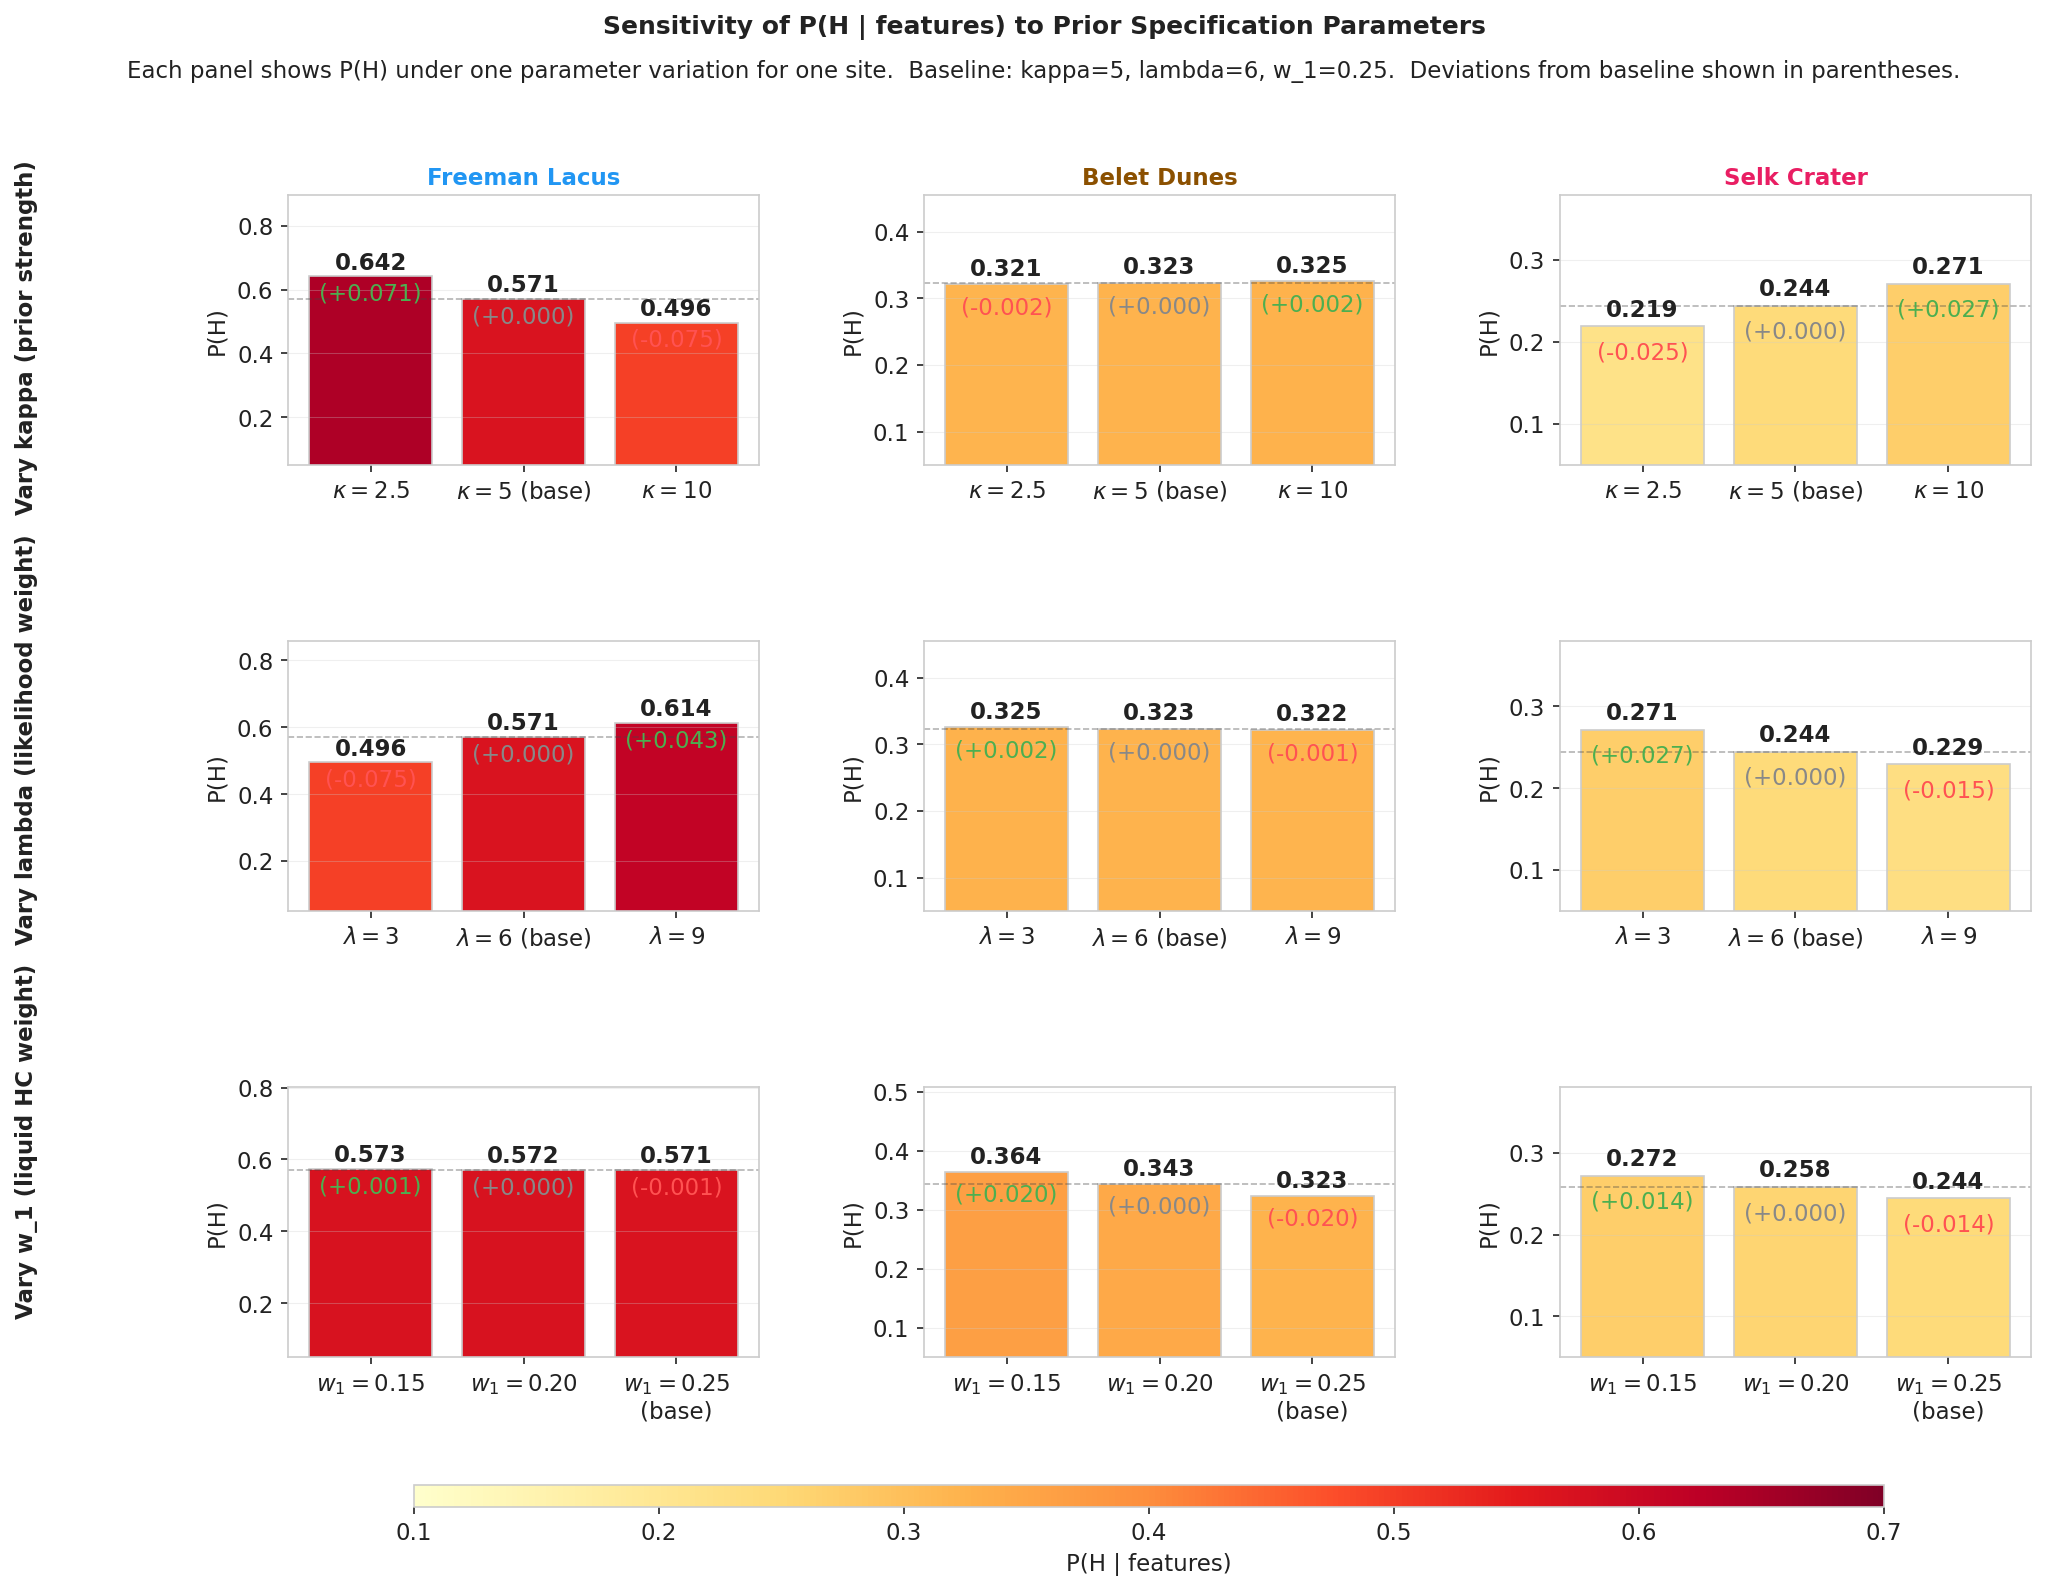
\includegraphics[width=\textwidth]{images/sensitivity_analysis.png}
  \caption{Sensitivity of $P(H\mid\mathbf{f})$ to prior specification.
    Each row varies one parameter; each column shows one site.
    All deviations $\leq 0.033$; qualitative rankings preserved across
    all 27 parameter combinations.}
  \label{fig:sensitivity}
\end{figure}

\section{Future Work}
\label{sec:future_work}

The three most impactful extensions are: (1)~post-\dragonfly{} recalibration of $f_2$ and $f_8$ weights using DraMS and DraGNS measurements at Selk; (2)~replacing the independence assumption with a full covariance structure estimated from high-resolution SAR patches; and (3)~additional temporal anchors at $-2.0$ to $-0.5\gya$ where the liquid-hydrocarbon ramp most sensitively determines whether equatorial or polar sites lead the transition.

\section{Conclusions}
\label{sec:conclusions}

This thesis presents the first quantitative, spatially-resolved, multi-epoch Bayesian habitability map of \titan{}'s surface, derived from eight Cassini observational proxy features.  Conclusions are organised by research question.

\paragraph{RQ1: Present-epoch spatial distribution.}
North polar lake margins are the most habitable present-day environments.  Kraken Mare's southern shoreline achieves $P(H)\approx0.44$ (rank~1), driven by coincident maximum $f_1{=}1.0$, $f_4{\approx}0.70$, and $f_7{\approx}0.76$.  All ten top-10 sites are lake or lacus margins; all eight feature-weight/importance ratios lie within 10\% of unity.

\paragraph{RQ2: LHB habitability.}
Cryovolcanic sites lead the \textit{Past} ranking (Hotei $P(H){=}0.295$) because their elevated $f_8$ and $f_5$ combine with the globally boosted acetylene proxy.  Craters rank 11th and below in the 8-feature formula; their astrobiological significance lies in providing transient liquid water for Strecker synthesis.

\paragraph{RQ3: Temporal trajectory.}
The trajectory is non-monotonic across three regimes.  (i)~LHB ($-3.8$ to $-1.5\gya$): cryovolcanic and impact-melt dominance, with tightly clustered scores reflecting the absence of a strong liquid-hydrocarbon signal.  (ii)~Polar-lake dominance ($-1.0$ to $+4.0\gya$): lake or lacus margins occupy all top-10 positions with stable rankings across three epochs; the present-day habitability structure is a plateau extending at least 250\,Myr into the future.  (iii)~Global ocean ($+5.1$ to $+6.0\gya$): all sites score $P(H){>}0.42$; cryovolcanic sites lead as their accumulated organic substrates dissolve into $\sim$10\,Gyr of photochemical product in warm water--ammonia.  A transient solvent-free minimum at $\sim$$+5.0\gya$ separates regimes (ii) and (iii).

\paragraph{RQ4: Dragonfly validation.}
Selk crater has the highest geodiversity of any equatorial site ($f_7{=}0.629$, $7.8\times$ the global median), derived independently from SAR data.  Its lower present-epoch score ($P(H){=}0.24$) is consistent: \dragonfly{} targets past water--organic chemistry, correctly identified by the two-framework distinction (Appendix~\ref{app:dragonfly}).

\bigskip
Together, these results demonstrate that \titan{} possesses a multilayered astrobiological significance from its geological past through the present to the far future, quantifiable from the Cassini dataset with sufficient precision to guide mission planning and interpret in-situ measurements.  The temporal reconstruction reveals a fundamental tension between habitability and abiogenesis (Section~\ref{sec:abiogenesis}): the sites with the highest present-day solvent habitability scores (polar lake shores) are the least understood in terms of origin-of-life potential, while the environments with the strongest abiogenesis credentials --- LHB impact-melt ponds and the red-giant ocean --- score modestly or lie in \titan{}'s temporal past and future respectively.
